\documentclass{article} % 文書クラスの指定
\usepackage[dvipdfmx]{graphicx}	      %	図を取り込む		   (推奨)
\usepackage{enumitem}                 %	箇条書きを変更する
% \usepackage{caption}                  % caption パッケージの追加
% \captionsetup[figure]{labelsep=} % 図のキャプションの形式を "図6.1(スペース)" に設定
% \captionsetup[table]{labelsep=space}  % 表のキャプションの形式を "表6.1(スペース)" に設定
\usepackage{color}                    % いろいろな色を使えるようにする
\usepackage{url}                      % URLを使えるようにする
\usepackage[left=20mm,right=20mm]{geometry}

% \usepackage{plistings}      % listingsパッケージをpLaTeX上で用いる際の日本語対応処理を強化するためのパッケージ.(plistings.sty)を同一ディレクトリに配置.

\title{音響信号への遅延生成アプリケーションの説明書} % 文書のタイトル
\author{知能信号処理研究室\\\\山下一樹} % 著者名
% 所属
% \date{\today} % 日付

\begin{document} % 文書の開始

\maketitle % タイトル、著者名、日付の表示
本稿は、身体運動への影響の調査で利用した「音響信号への遅延生成アプリケーション」を使用するための説明書です。
本稿の内容がアプリケーションの使用や改善の際に少しでも役立てば幸いです。
\section{各要素の説明} 
Figure \ref{fig:app_kyakkann}にアプリケーションの画面の一例を示します。
以下に赤色の点線で囲った画面内の各要素について説明します。
ここで述べられるデフォルトの設定値は、アプリケーションを起動した際のデフォルトの設定値です。「window.cpp」を編集することで変更できます。
\begin{figure}[tbp]
  \centering
  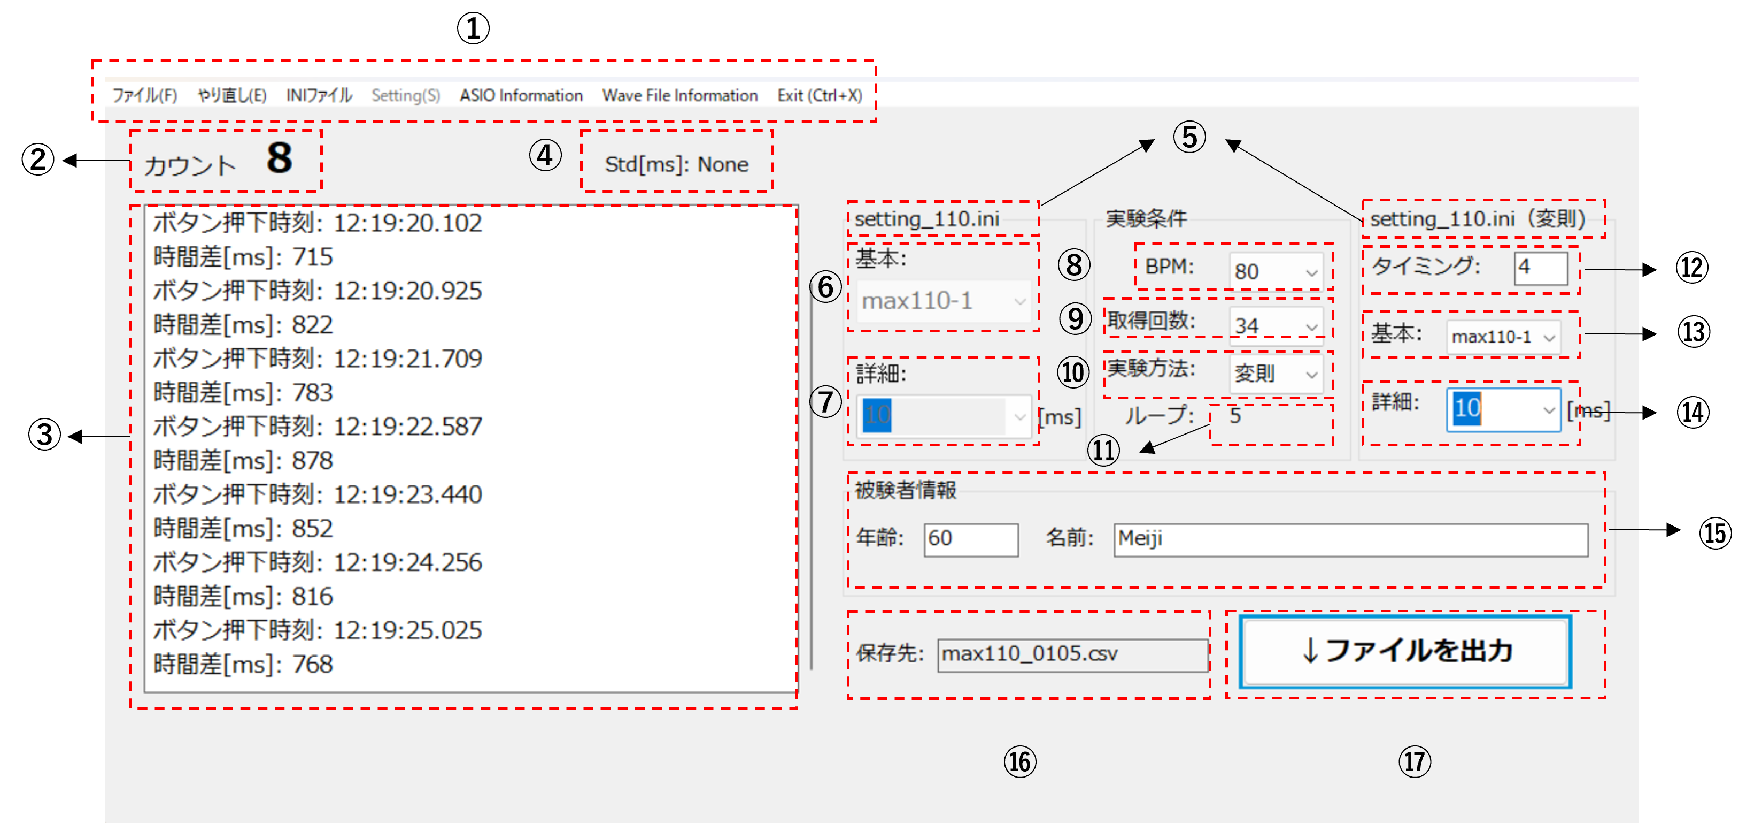
\includegraphics[scale=0.5]{figures_app_1.pdf}
  \caption{アプリケーションの画面の一例}
  \label{fig:app_kyakkann}
\end{figure}
\begin{enumerate}[label=(\arabic*), leftmargin=*]
  \item メニューバーです。アプリケーションの操作に関するメニューが表示されます。
  「ファイル」は、結果を保存するためのCSVファイルを選択するためのメニューです。
  「やり直し」は、ボタンの押下回数をリセットするためのメニューです。
  「INIファイル」は、遅延時間が記述されているiniファイルを選択するメニューです。このiniファイルは指定されたフォルダ内に保存されている必要があります。詳細は2章を参照してください。
  \item ボタンの押下回数を表示します。
  \item ボタンの押下時刻と前回押した時刻との差[ms]を表示します。 
  \item ボタンの押下時間間隔[ms]のデータの標準偏差を表示します。外れ値を含むすべてのデータの標準偏差を表示します。
  分析データとしてはこの値は使用しません。
  \item 設定したiniファイル名を表示します。
  \item 指定したiniファイルに記述された遅延時間のグループ名を表示するコンボボックス。
  \item (6)で選択された遅延時間のグループ名の遅延時間[ms]を表示するコンボボックス。
  \item CSVファイルに出力するBPMの値を指定するためのコンボボックス。デフォルトは80です。
  \item ボタンの押下時間間隔の取得回数を指定するためのコンボボックス。デフォルトは34です。(2)がここで指定した回数に到達すると、
  メッセージボックスが出力され音の出力が一時的に停止します。
  \item 実験方法を指定するためのコンボボックス。デフォルトは「変則」です。
  変則に設定すると、右側のコンボボックスが有効化されます。通常の場合、常に(7)で設定した遅延時間でクリック音が出力されます。
  変則の場合、ボタンの押下回数が(12)で指定した倍数に到達するとクリック音に遅延が(14)で指定した遅延時間だけ加えられた状態で出力されます。
  ボタンの押下回数が(12)で指定した倍数ではない場合は、(7)で指定した時間だけクリック音に遅延が加えられた状態で出力されます。
  \item プログラム中で設定するfor分のループ回数。この値が小さい程遅延時間が小さいです。動作確認用で使用していたため、実験では使用していません。
  \item 遅延のタイミングを指定するためのエディットボックス。デフォルトは4です。ここで指定された値の倍数に(2)が到達するとクリック音に遅延が(14)で指定した遅延時間だけ加えられます。
  \item (1)で設定したiniファイルのグループ名を指定するためのコンボボックス。
  \item (13)で指定したグループの遅延時間[ms]を指定するためのコンボボックス。
  \item 被験者の情報を入力するためのエディットボックス。ここに書かれた情報もCSVファイルに書き込まれます。
  後続のデータ整理の時などに利用しました。
  \item (1)で選択したCSVファイルの名前を表示します。
  \item 結果を保存するためのプッシュボタン。押下すると、(1)で指定したCSVファイルに結果がカンマ区切りで書き込まれ、保存されます。(10)で指定した実験方法により、書き込まれるデータの内容が若干異なります。書き込まれるデータの内容を以下に示します。
  \begin{enumerate}
    \item 実験方法が「変則」の場合
    
    irregular,ボタンの押下回数が(12)で指定した数の倍数の時に発生する遅延時間[ms],遅延が発生するタイミング, データを取得した日付,ボタンの押下回数が(12)で指定した数以外の倍数の時に発生する遅延時間[ms],遅延時間のグループ名,被験者の名前,年齢,BPM,ボタンの押下時間間隔のデータ[ms]
    \item 実験方法が「通常」の場合
    
    データを取得した日付,遅延時間[ms],遅延時間のグループ名,被験者の名前,年齢,BPM,ボタンの押下時間間隔のデータ[ms]
  \end{enumerate}
\end{enumerate}
\newpage
\section{INIファイルの設定}
Figure \ref{fig:ini-file}にiniファイルの例を示します。
アプリケーションがiniファイルに記述された遅延時間を読み込むために、exeファイルと同じフォルダ内に、
「setting」という名前のフォルダを作成し、その中に遅延時間を記述したiniファイルを保存する必要があります。
setting\_110.iniファイルに遅延時間を設定しておくことができます。iniファイルはテキストエディタで編集可能です。
以下にiniファイルの例を示します。
まず、「setting」セクション内の「latedataname」キーに遅延時間のグループ名を設定します。
次に、設定した遅延時間のグループ名のセクションを作成し、「data」キーにカンマ区切りで遅延時間を設定します。
これを行うとアプリケーションで遅延時間を読み込むことができます。
\begin{figure}[tbp]
  \centering
  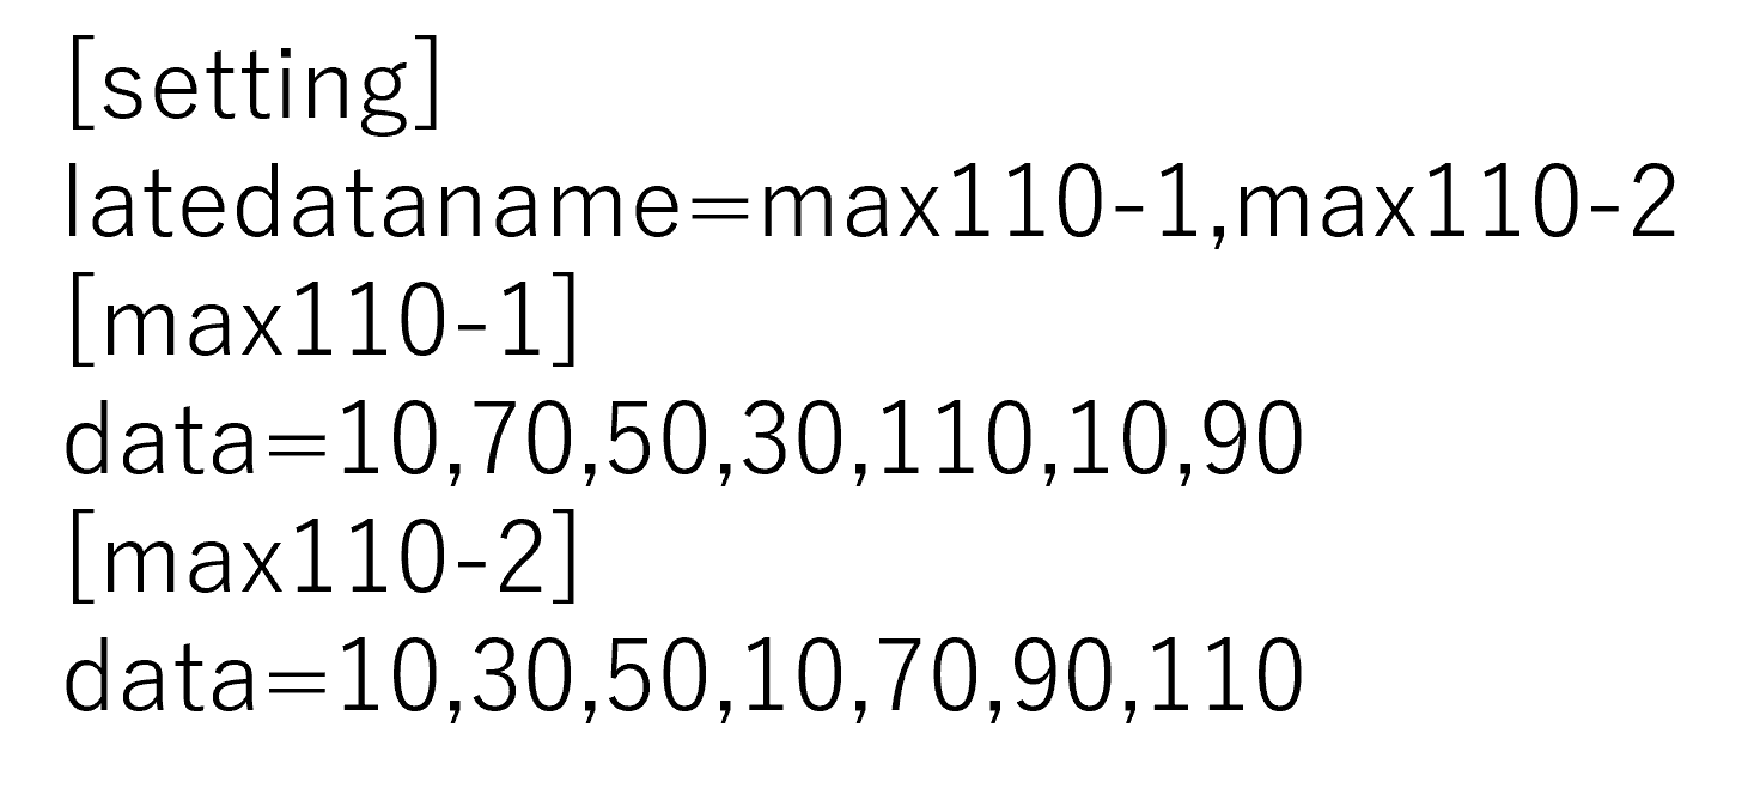
\includegraphics[scale=0.3]{setting-ini.pdf}
  \caption{setting\_110.iniの例}
  \label{fig:ini-file}
\end{figure}

% \section{改善すべき点}
% 以下にこのアプリケーションの改善すべき点を示します。
% \begin{enumerate}
%   \item iniファイルのデフォルト名が「setting\_110.ini」になっている。そのため、決まったフォルダ内に「setting\_110.ini」が保存されていなければならない。どんな名前のiniファイルでも読み込めるようにする。
%   \item 音声の出力先のチャンネル数を指定できるようにする。
%   \item ボタンの押下回数が指定された回数に到達したときに、メッセージボックスによって強制的に音声の出力を一時的に停止する機能があるが、
%   メッセージボックスを閉じた直後に音声が出力されないようにしたい。
% \end{enumerate}
\end{document} % 文書の終了
